\section{Aspect médical}

\begin{frame}
\tableofcontents[currentsection, hideothersubsections]
\end{frame}

\begin{frame}{Pré-requis}
	\begin{block}{Projet multidisciplinaire}
		\begin{itemize}
			\item Acquérir les connaissances médicales de base  \pause
			\item Comprendre les enjeux et le contexte médico-social  \pause
			\item Analyser quels peuvent être les besoins
		\end{itemize}			
	\end{block}  \pause
		\begin{block}{Étude de terrain}
		\begin{itemize}
			\item Recherche et études documentaires  \pause
			\item Premières suppositions   \pause
			\item Rencontrer patient et professionnels  \pause
			\item Confronter les idées
		\end{itemize}			
	\end{block}
\end{frame}

\begin{frame}{Fugl-Meyer assessment Sensorimotor Recovery after Stroke}
	\begin{block}{Définition}
Mesure de la déficience moteur et sensorielle des membres supérieurs et inférieurs.
	\end{block}  \pause
	\begin{block}{Description}
Constitue un ensemble d'exercices dont chaque mouvement est évalué selon 1 ou plusieurs critères, permettant une évaluation de la sensibilité, du tonus, de la force et de la motricité du patient à travers l'analyse de son score.
	\end{block}
\end{frame}

\begin{frame}{Fugl-Meyer assessment}
	\begin{block}{Fonctionnement}
		Découpage permettant d'obtenir 3 sous-scores : 
		\begin{itemize}
			\item membre supérieur : 33 items, coté 0 à 66
			\item membre inférieur : 17 items, coté 0 à 34
			\item équilibre : 7 items, coté 0 à 14
		\end{itemize}
	\end{block}  \pause
	\begin{block}{Précision}
		Décomposition de  la partie membre supérieur en 2 sections : 
		\begin{itemize}
			\item score distal \footnote{partie d’un membre la plus éloignée de la base de celui-ci} 
			\item score proximal\footnote{partie du corps proche de la racine d’un membre}
		\end{itemize}
	\end{block}	
\end{frame}

\begin{frame}{Fugl-Meyer assessment}
	\begin{figure}
	\centering
	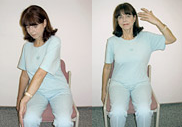
\includegraphics[width=6cm]{../images/fuglmeyer_example.png}
	\caption{Exemple d’un exercice du membre supérieur du test de Fugl-Meyer}
	\end{figure}
\end{frame}

\begin{frame}{L'avis des professionnels}
L'échelle sensorimotrice de Fugl Meyer :
	\begin{exampleblock}{Avantages}
			\begin{itemize}
			\item Constitue le "Gold Standard"  \pause
			\item Très utilisée en recherche et dans la littérature 
		\end{itemize}  \pause
	\end{exampleblock}
	\begin{alertblock}{Critiques}
			\begin{itemize}
			\item Variabilités des résultats : imprécision des mesures, subjectivité de la notation  \pause
			\item Faible amplitude de mesure : effet "plateau", pas représentatif des progrès   \pause
			\item Test de déficiences et non fonctionnel
		\end{itemize}
	\end{alertblock}	
\end{frame}